% igs2ejournalguide.tex
% v4.00 3-sept-2015

\NeedsTeXFormat{LaTeX2e}

% check that the math fits the two-column format:
 \documentclass[twocolumn, letterpaper]{igs}

% but use this version when submitting your article:
% \documentclass[review,oneside, letterpaper]{igs}

  \usepackage{igsnatbib}
  \usepackage{lmodern}
\usepackage{amsmath,amssymb,amsthm}
\usepackage{wrapfig}
\usepackage{enumitem}
\usepackage{multirow}
\usepackage{tabularx}
\usepackage{booktabs}
\usepackage{lscape}
\usepackage{caption,threeparttable}
\usepackage{dblfloatfix}
\usepackage{color}

\newcolumntype{C}{>{\centering\arraybackslash}X}
\renewcommand{\tabularxcolumn}[1]{m{#1}}%


% check if we are compiling under latex or pdflatex
  \ifx\pdftexversion\undefined
    \usepackage[dvips]{graphicx}
  \else
    \usepackage[pdftex]{graphicx}
    \usepackage{epstopdf}
    \epstopdfsetup{suffix=}
  \fi


\begin{document}

\title[]{Estimating winter balance and its uncertainties from direct measurements of snow depth and density on alpine glaciers}

\author[]{Alexandra PULWICKI,$^1$
  Gwenn E. FLOWERS,$^1$ Valentina  RADI\'C,$^2$}

\affiliation{%
$^1$ Department of Earth Sciences, Faculty of Science, Simon Fraser University, Burnaby, BC, Canada\\
$^2$Department of Earth, Ocean and Atmospheric Sciences, Faculty of Science, University of British Columbia, Vancouver, BC, Canada\\
  Correspondence: Alexandra Pulwicki 
  $<$apulwick@sfu.ca$>$}


%%%%%%%%%%%%%%%%%%%%%%%%%%%%%%%%%
%	ABSTRACT
%%%%%%%%%%%%%%%%%%%%%%%%%%%%%%%%%

\abstract{Accurately estimating winter surface mass balance on glaciers is central to assessing glacier health and predicting glacier runoff. However, measuring and modelling snow distribution is inherently difficult in mountainous terrain, resulting in high uncertainties in estimates of winter balance. \textcolor{red}{In this study, we explore rigorous statistical methods of estimating winter balance and its uncertainty from direct measurements of snow depth and density at multiple scales.} We collected more than 9000 direct measurements of snow depth across three glaciers in the St. Elias Mountains, Yukon, Canada in May 2016. Linear regression and simple kriging, combined with cross correlation and Bayesian model averaging, are used to interpolate point-scale winter balance estimates across the glacier. Elevation and a simple wind-redistribution parameter are found to be the dominant controls on the spatial distribution of winter balance, but the relationship varies considerably between glaciers. Through a Monte Carlo analysis, we find that the interpolation of winter balance values is a larger source of uncertainty than the assignment of snow density or than the \textcolor{red}{subgrid variability}. For our study glaciers, the \textcolor{red}{winter balance uncertainty from all assessed sources} ranges from 0.03\,m\,w.e. (8\%) to 0.15\,m\,w.e. (54\%) depending primarily on the interpolation method. Despite the challenges associated with estimating winter balance, our results are consistent with a regional-scale winter-balance gradient. (220 words) }

\maketitle




%%%%%%%%%%%%%%%%%%%%%%%%%%%%%%%%%
%	INTRODUCTION
%%%%%%%%%%%%%%%%%%%%%%%%%%%%%%%%%
\section{Introduction}

Winter surface mass balance, or ``winter balance'', is the net accumulation and ablation of snow over the winter season \citep{Cogley2011}, which constitutes glacier mass input. \textcolor{red}{Winter balance is half of the seasonally resolved mass balance, initializes summer ablation conditions, and ...} \citep[e.g.][]{Hock2005,Reveillet2016}. Effectively representing the spatial distribution of snow is also important for modelling energy and mass exchange between the land and atmosphere, allowing for better monitoring of surface runoff and its downstream effects \citep[e.g.][]{Clark2011}.

Winter balance (WB) is notoriously difficult to estimate. Snow distribution in alpine regions is highly variable with short correlation length scales \citep[e.g.][]{Anderton2004, Egli2011, Grunewald2010, Helbig2017, Lopez2011, Lopez2013, Machguth2006, Marshall2006} and is influenced by dynamic interactions between the atmosphere and complex topography, operating on multiple spatial and temporal scales \citep[e.g.][]{Barry1992, Liston2006, Clark2011}. Simultaneously extensive, high resolution and accurate snow distribution measurements on glaciers are therefore almost impossible to obtain \citep[e.g.][]{Cogley2011, McGrath2015}. Further, current models are computationally intensive and sensitive to initial conditions so there is a significant source of uncertainty that undermines the ability of models to represent current and projected glacier conditions. FIX ME

Studies that have focused on obtaining detailed estimates of WB have used a wide range of observational techniques, including direct measurement of snow depth and density \citep[e.g.][]{Cullen2017}, lidar or photogrammerty \citep[e.g.][]{Sold2013} and ground-penetrating radar \citep[e.g.][]{Machguth2006, Gusmeroli2014, McGrath2015}. Spatial coverage of direct measurements is generally limited and often comprises an elevation transect along the glacier centreline \citep[e.g.][]{Kaser2003}. Measurement are often interpolated using a linear regression on only a few topographic parameters \citep[e.g.][]{MacDougall2011}, with elevation being the most common. Other established techniques include hand contouring \citep[e.g.][]{Tangborn1975}, kriging \citep[e.g.][]{Hock1999} and attributing measured winter balance values to elevation bands \citep[e.g.][]{Thibert2008}. Physical snow models have been used to estimate spatial patterns of winter balance \citep[e.g.][]{Mott2008, Schuler2008, Dadic2010} but limited meteorological data generally prohibits their wide spread application. Error analysis is rarely undertaken and few studies have thoroughly investigated uncertainty in spatially distributed estimates of winter balance estimates \citep[c.f.][]{Schuler2008}. 

\textcolor{red}{More sophisticated snow survey designs and statistical models of snow distribution are available and widely used in the field of snow science.} Surveys described in the snow science literature are generally spatially extensive and designed to measure snow depth and density throughout a basin, ensuring that all terrain types are sampled. A wide array of measurement interpolation methods are used, including linear \citep[e.g.][]{Lopez2010} and non-linear regressions \citep[e.g.][]{Molotch2005} that include numerous terrain parameters, as well as geospatial interpolation \citep[e.g.][]{Erxleben2002} including various forms of  kriging. Different interpolation methods are often combined (e.g. regression kriging) to yield improved fits \citep[e.g.][]{Balk2000}. Physical snow models such as Alpine3D \citep{Lehning2006} and SnowDrift3D \citep{Schneiderbauer2011} are widely used in snow science, and errors in estimating snow distribution have been examined from theoretical \citep[e.g.][]{Trujillo2015} and applied perspectives \citep[e.g.][]{Turcan1975,Woo1978, Deems2006}. 

The goals of this study are to (1) critically examine methods of converting direct snow depth and density measurements to distributed estimates of winter balance and to (2) identify sources of uncertainty, evaluate their magnitude and assess their combined contribution to uncertainty in glacier-wide winter balance. We focus on commonly applied, low-complexity methods of measuring and estimating winter balance in the interest of making our results broadly applicable.


%%%%%%%%%%%%%%%%%%%%%%%%%%%%%%%%%
%	STUDY SITE
%%%%%%%%%%%%%%%%%%%%%%%%%%%%%%%%%
\begin{figure*}
	\centering
	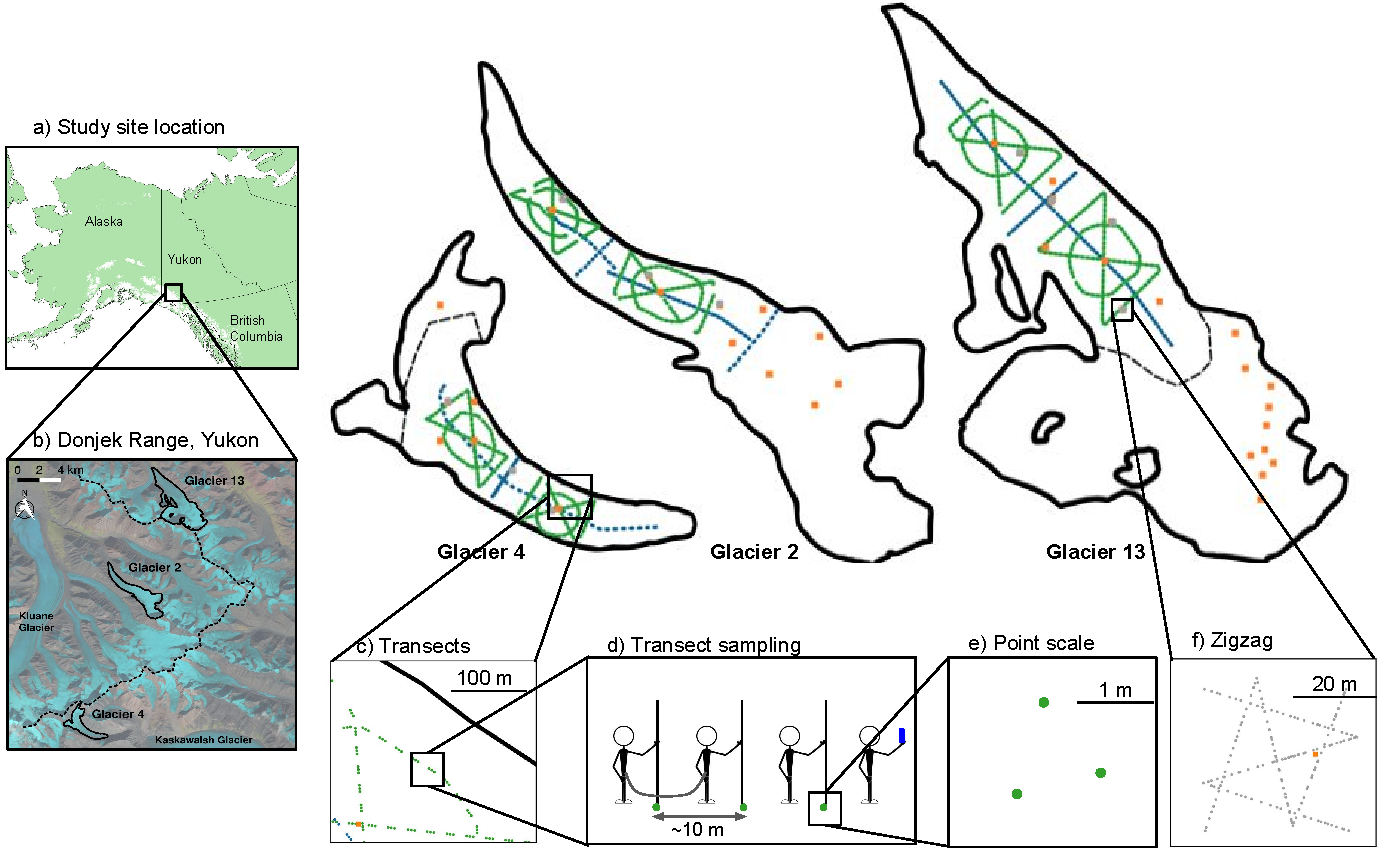
\includegraphics[width =0.9\textwidth]{Sampling.pdf}\\
	\caption{Study area location and sampling design for Glaciers 4, 2 and 13. (a) Study region in the Donjek Range of the St. Elias Mountains of Yukon, Canada. (b) Study glaciers located along a southwest-northeast transect through the Donjek Range. The local topographic divide is shown as a dashed line. Imagery from Landsat8 (5 September 2013, data available from the U.S. Geological Survey). (c) Details of the snow-survey sampling design, with centreline and transverse transects (blue dots) and hourglass and circle designs (green dots) and locations of snow density measurements (orange squares). Arrows indicate glacier flow direction. Approximate location of ELA is shown as a black dashed line. (d) Close up of linear and curvilinear transects. \textcolor{red}{(e) Configuration of observers. (f) Point-scale snow depth sampling.}(g) Linear-random snow-depth measurements in `zigzag' design (grey dots) with one density measurement (orange square) per zigzag.}
	\label{fig:Sampling}
\end{figure*}

\section{Study site}

The St. Elias Mountains (Fig. \ref{fig:Sampling}a) rise sharply from the Pacific Ocean, creating a significant climatic gradient between coastal maritime conditions, generated by Aleutian--Gulf of Alaska low-pressure systems, and interior continental conditions, driven by the Yukon--Mackenzie high-pressure system \citep{Taylor1969}. The boundary between the two climatic zones is generally aligned with the divide between the Hubbard and Kaskawulsh Glaciers, approximately 130\,km from the coast. The Donjek Range is located approximately 40 km to the east of this divide. Research on snow distribution and glacier mass balance in this area is limited. \textcolor{red}{A series of research programs, including Project ``Snow Cornice''  and the Icefield Ranges Research Project, were operational in the 1950s and 60s \citep{Wood1948, Danby2003} and in the last 30 years, there have been a few long-term studies on select alpine glaciers \citep{Clarke2014}.}

Winter balance surveys were conducted on three glaciers in the Donjek Range of the St. Elias Mountains. The Donjek Range is approximately $30\times30$ km and Glacier 4, Glacier 2 and Glacier 13 (labelling adopted from \cite{Crompton2016}) are located along a southwest-northeast transect through the range (Fig. \ref{fig:Sampling}b, Table \ref{tab:GlacierDetails}). These small, polythermal alpine glaciers are generally oriented southeast-northwest, with Glacier 4 having a predominantly southeast facing aspect and Glaciers 2 and 13 have generally northwest facing aspects. The glaciers are situated in valleys with steep walls have simple geometries. 


\begin{table*}[]
\centering
\caption{Physical characteristics of study glaciers and May 2016 winter-balance survey details for study glaciers, including number of snow-depth measurement locations along transects ($n_{\mathrm{T}}$), total length of transects ($d_{\mathrm{T}}$), number of combined snow pit (SP) and Federal Sampler (FS) density measurement locations ($n_{\rho}$) and number of zigzag surveys ($n_{\mathrm{zz}}$).}
\label{tab:GlacierDetails}
\begin{tabular}{cccccccccccc}
\midrule
\textbf{} & \textbf{Location} & \multicolumn{3}{c}{\textbf{Elevation (m a.s.l)}} & \textbf{Slope ($^{\circ}$)} & \multirow{2}{*}{\textbf{\begin{tabular}[c]{@{}c@{}}Area\\ (km)\end{tabular}}} & \multirow{2}{*}{\textbf{\begin{tabular}[c]{@{}c@{}}Survey\\ Dates\end{tabular}}} & \multicolumn{4}{c}{\textbf{Survey Details}} \\
 & UTM Zone 7 & \textit{Mean} & \textit{Range} & \textit{ELA} & \textit{Mean} &  &  & $n_{\mathrm{T}}$ & $d_{\mathrm{T}}$ (km) & $n_{\rho}$ & $n_{\mathrm{zz}}$ \\ \midrule
\textbf{Glacier 4} & \begin{tabular}[c]{@{}c@{}}595470 E\\ 6740730 N\end{tabular} & 2344 & 1958--2809 & $\sim$2500 & 12.8 & 3.8 & 4--7 May 2016 & 649 & 13.1 & 10 & 3 \\
\textbf{Glacier 2} & \begin{tabular}[c]{@{}c@{}}601160 E\\ 6753785 N\end{tabular} & 2495 & 1899--3103 & $\sim$2500 & 13.0 & 7.0 & 8--11 May 2016 & 762 & 13.6 & 11 & 3 \\
\textbf{Glacier 13} & \begin{tabular}[c]{@{}c@{}}604602 E\\ 6763400 N\end{tabular} & 2428 & 1923--3067 & $\sim$2380 & 13.4 & 12.6 & 12--15 May 2016 & 941 & 18.1 & 20 & 4
\end{tabular}
\end{table*}

%%%%%%%%%%%%%%%%%%%%%%%%%%%%%%%%%
%	METHODS
%%%%%%%%%%%%%%%%%%%%%%%%%%%%%%%%%


\section{Methods}

\textcolor{red}{Estimating glacier-wide WB involves transforming measurements of snow depth and density into distributed winter balance across a defined grid.} We do this in four steps. (1) Obtain direct measurements of snow depth and density in the field. (2) Assign density values to all depth-measurement locations to calculate point-scale WB at each location. (3) Average all point-scale WB values within each gridcell of a digital elevation model (DEM) to obtain the gricell-averaged WB. (4) Interpolate and extrapolate these gridcell-averaged WB values to obtain estimates of WB (in\,m\,w.e.) in each gridcell across the domain. \textcolor{red}{In Step 4, we use linear regression between gridcell-averaged WB and various topographic parameters because this method has precedent for success \citep[e.g.][]{McGrath2015}. Instead of a basic regression, we use cross-validation and model averaging to test all combinations of the chosen topographic parameters.We compare the regression approach with simple kriging (SK), a data-driven interpolation method, to interpolate WB in Step 4 without invoking physical interpretation \citep[e.g.][]{Hock1999}.} For brevity, we refer to these four steps as (1) field measurements, (2) density assignment, (3) gridcell-averaged WB and (4) distributed WB. Detailed methodology for each step is outlined below.

\subsection{Field measurements}

\subsubsection{Sampling design}

The snow surveys were designed to capture variability in snow depth at regional, basin, gridcell and point scales \citep{Clark2011}. To capture variability at the regional scale we chose three glaciers along the dominant precipitation gradient in the St. Elias Mountains, Yukon (Fig. \ref{fig:Sampling}) \citep{Taylor1969}. To account for basin-scale variability, snow depth was measured along linear and curvilinear transects on each glacier (Fig. \ref{fig:Sampling}c) with sample spacing of $10-60$ m (Fig. \ref{fig:Sampling}d). \textcolor{red}{Sample spacing was constrained by protocols for safe glacier travel, while survey scope was constrained by the need to complete surveys on all three glaciers within the period of peak accumulation.} We selected centreline and transverse transects as the most commonly used survey in winter balance studies \citep[e.g.][]{Kaser2003, Machguth2006} as well as an hourglass pattern with an inscribed circle, which allows for sampling in multiple directions and easy travel (personal communication from C. Parr, 2016). To capture variability at the grid scale, we densely sampled up to four gridcells on each glacier using a linear-random sampling design we term `zigzag'. To capture point-scale variability, each observer made 3--4 depth measurements within $\sim$1 m of each other (Fig. \ref{fig:Sampling}e) at each transect measurement location. In total, we collected more than 9000 snow depth measurements throughout the study area (Table \ref {tab:GlacierDetails}). 

\subsubsection{Snow depth: transects}

Winter balance can be estimated as the product of snow depth and depth-averaged density. Snow depth is generally accepted to be more variable than density \citep{Elder1991, Clark2011, Lopez2013} so we chose a sampling design that resulted in a high ratio ($\sim$55:1) snow depth to density measurements. Our sampling campaign involved four people and occurred between 5--15 May 2016, corresponding to the peak seasonal snow accumulation in Yukon (Yukon Snow Survey Bulletin and Water Supply Forecast, May 1, 2016). While roped-up for glacier travel at fixed distances between observers, the lead observer used a single-frequency GPS unit (Garmin GPSMAP 64s) to navigate between predefined transect measurement locations (Fig. \ref{fig:Sampling}e). The remaining three observers used 3.2 m graduated aluminium avalanche probes to make snow depth measurements. The locations of each set of depth measurements, made by the second, third and fourth observers, are estimated using the recorded location of the first observer, the known distance between observers and the direction of travel. 

Snow-depth sampling was concentrated in the ablation area to ensure that only snow from the current accumulation season was measured. The boundary between snow and firn in the accumulation area can be difficult to detect and often misinterpreted, especially when using an avalanche probe \citep{Grunewald2010,Sold2013}. We intended to use a firn corer to measure winter balance in the accumulation area, but cold snow combined with positive air temperatures led to cores being unrecoverable. Successful snow depth and density measurements within the accumulation area were made either in snow pits or using a Federal Sampler to unambiguously identify the snow--firn transition. 

\subsubsection{Snow depth: zigzags}

To capture snow-depth variability within a single DEM gridcell, we implemented a linear-random zigzag sampling design \citep{Shea2010}. \textcolor{red}{We measured depth at random intervals of 0.3--3.0\,m along two `Z'-shaped patterns, resulting in 135--191 measurements, within three to four $40\times40$ m gridcells (Fig. \ref{fig:Sampling}g) per glacier. Random intervals had a uniform distribution and were generated in MATLAB.} Zigzag locations were randomly chosen within the upper, middle, and lower regions of the ablation area of each glacier. We were able to measure a fourth zigzag on Glacier 13 that was located in the central ablation area, $\sim$2200 m a.s.l.

\subsubsection{Snow density}

Snow density was measured using a Snowmetrics wedge cutter in three snow pits on each glacier, as well as with a \textcolor{red}{Geo Scientific Ltd. metric Federal Sampler}. Within the snow pits (SP), we measured a vertical density profile (at 5 cm increments) with the $5\times10\times 10$ cm wedge-shaped cutter (250 cm$^3$) and a Presola 1000\,g spring scale \citep[e.g.][]{Gray1981,Fierz2009}. Uncertainty in estimating density from snow pit measurements stems from incorrect assignment of density to layers that cannot be sampled (e.g. ice lenses and hard layers). We attempt to quantify this uncertainty by varying estimated ice layer thickness by $\pm$1 cm ($\leq$100\%) of the recorded thickness, ice layer density between 700 and 900\,kg\,m$^{-3}$ and the density of layers identified as being too hard to sample (but not ice) between 600 and 700\,kg\,m$^{-3}$. When considering all three sources of uncertainty, the range of integrated density values is always less than 15\% of the reference density. Depth-averaged densities for shallow pits ($<$50\,cm) that contain ice lenses are particularly sensitive to changes in prescribed density and ice-lens thicknesses. 

While snow pits provide the most accurate measure of snow density, digging and sampling a snow pit is time and labour intensive. Therefore, a Federal Snow Sampler (FS) \citep{Clyde1932}, which directly measures depth-integrated snow-water equivalent, was used to augment the snow pit measurements. A minimum of three Federal Sampler measurements were taken at each of $7-19$ locations on each glacier and an additional eight Federal Sampler measurements were co-located with each snow pit profile. Measurements for which the snow core length inside the sampling tube was less than 90\% of the snow depth were discarded. \textcolor{red}{Density values at each measurement location (eight at snow pit locations, three elsewhere) were then averaged to obtain the uncertainty, which is taken to be the standard deviation of these measurements.}

During the field campaign there were two small accumulation events. The first, on 6 May 2016, also involved high winds so accumulation could not be determined. The second, on 10 May 2016, resulted in 0.01 m w.e accumulation measured at one location on Glacier 2. Positive temperatures and clear skies occurred between 11--16 May 2016, which we suspect resulted in melt occurring on Glacier 13. The snow in the lower part of the ablation area of Glacier 13 was isothermal and showed clear signs of melt and metamorphosis. The total amount of accumulation and melt during the study period could not be estimated so no corrections were made. 

\subsection{Density assignment}

Measured snow density must be interpolated or extrapolated to estimate point-scale winter balance at each snow-depth sampling location. We employ four commonly used methods to interpolate and extrapolate density (Table \ref{tab:densityOptions}): (1) calculate mean density over an entire mountain range \citep[e.g.][]{Cullen2017}, (2) calculate mean density for each glacier \citep[e.g.][]{Elder1991, McGrath2015}, (3) linear regression of density on elevation for each glacier \citep[e.g.][]{Elder1998, Molotch2005} and (4) calculate mean density using inverse-distance weighting \citep[e.g.][]{Molotch2005} for each glacier.  SP- and FS-derived densities are treated separately, for reasons explained below, resulting in eight possible methods of assigning density.

\begin{table}
\centering
\caption{Eight methods used to estimate snow density at unmeasured locations for purpose of converting measured snow depth to point-scale winter balance.}
\label{tab:densityOptions}
\begin{tabular}{cccc}
\hline
\multirow{2}{*}{\textbf{\begin{tabular}[c]{@{}c@{}}Method \\ code \end{tabular}}} & \multicolumn{2}{c}{\textbf{\begin{tabular}[c]{@{}c@{}}Source of measured \\ snow density\end{tabular}}} & \multirow{2}{*}{\textbf{\begin{tabular}[c]{@{}c@{}}Density assignment \\ method\end{tabular}}} \\
 & \textit{Snow pit} & \textit{\begin{tabular}[c]{@{}c@{}}Federal\\ Sampler\end{tabular}} &  \\ \hline
S1 & $\blacksquare$ &  & \multirow{2}{*}{\begin{tabular}[c]{@{}c@{}}Mean of measurements \\ across all glaciers\end{tabular}} \\
F1 &  & $\blacksquare$ &  \\ \hline
S2 & $\blacksquare$ &  & \multirow{2}{*}{\begin{tabular}[c]{@{}c@{}}Mean of  measurements \\ within a given glacier\end{tabular}} \\
F2 &  & $\blacksquare$ &  \\ \hline
S3 & $\blacksquare$ &  & \multirow{2}{*}{\begin{tabular}[c]{@{}c@{}}Regression of density on \\ elevation within a glacier\end{tabular}} \\
F3 &  & $\blacksquare$ &  \\ \hline
S4 & $\blacksquare$ &  & \multirow{2}{*}{\begin{tabular}[c]{@{}c@{}}Inverse distance \\ weighted mean\end{tabular}} \\
F4 &  & $\blacksquare$ & 
\end{tabular}
\end{table}
 

\subsection{Gridcell-averaged winter balance}

We average one to six (mean of 2.1 measurements) point-scale values of WB within each $40 \times 40$ m DEM gridcell to obtain the gricell-averaged WB. The locations of individual measurements have  uncertainty due to the error in the horizontal position given by the GPS unit and the estimation of observer location based on the recorded GPS positions of the navigator. This location uncertainty could result in the incorrect assignment of a point-scale WB to a particular gridcell. However, this source of error is not further investigated because we assume that the uncertainty in gridcell-averaged WB is captured in the zigzag measurements described below. \textcolor{red}{Uncertainty due to having multiple observers was also tested. There are no significant differences between snow depth measurements made by observers along a transect (p$>$0.05), with the exception of the first transect on Glacier 4 (51 measurements)}. 

\subsection{Distributed winter balance}

\subsubsection{Linear regression}

Gridcell-averaged values of WB are interpolated and extrapolated across each glacier using linear regression (LR) and simple kriging (SK). The regression relates gridcell-averaged values of WB to DEM-derived topographic parameters. We use commonly applied topographic parameters as in \cite{McGrath2015}, including elevation, slope, aspect, curvature, ``northness'' and a wind-redistribution parameter; we add distance-from-centreline as an additional parameter. Our sampling design ensured that the ranges of topographic parameters associated with our measurement locations represent more than 70\% of the total area of each glacier (except elevation on Glacier 2, where our measurements captured only 50\%). Topographic parameters are weighted by a set of fitted regression coefficients ($\beta_i$) calculated by minimizing the sum of squares of the vertical deviations of each datum from the regression line \citep{Davis1986}. For details on data and methods used to estimate the topographic parameters see the Supplementary Material. 

To avoid overfitting the data and to \textcolor{red}{ incorporate every possible combination of topographic parameters}, cross-validation and model averaging are implemented. First, cross-validation is used to obtain a set of $\beta_i$ values that have the greatest predictive ability. We randomly select 1000 subsets of the data (2/3 of the values) to fit the LR and use the remaining data (1/3 of the values) to calculate a root mean squared error (RMSE) \citep{Kohavi1995}. Regression coefficients resulting in the lowest RMSE (1000 values) are selected. Second, we use model averaging to account for uncertainty when selecting predictors and to maximize the model's predictive ability \citep{Madigan1994}.  \textcolor{red}{Models are generated by calculating a set of $\beta_i$ for all possible combinations of topographic parameters (2$^7$ models).} Following a Bayesian framework, model averaging involves weighting all models by their posterior model probabilities \citep{Raftery1997}. To obtain the final regression coefficients, the $\beta_i$ values from each model are weighted according to the relative predictive success of the model, as assessed by the value of the Bayesian Information Criterion (BIC) \citep{Burnham2004}. BIC penalizes more complex models which further reduces the risk of overfitting. The distributed WB is then obtained by applying the resulting regression coefficients to the topographic parameters associated with each gridcell. 

\subsubsection{Simple kriging}

Simple kriging (SK) is a data-driven method of estimating variables at unsampled locations by using the isotropic spatial correlation (covariance) of measured values to find a set of optimal weights \citep{Davis1986, Li2008}. Simple kriging assumes spatial correlation between sampling locations that are distributed across a surface and then applies the correlation to interpolate between these locations. We used the \texttt{DiceKriging} R package \citep{Roustant2012} to calculate the maximum likelihood covariance matrix, as well as the range distance ($\theta$) and nugget for gridcell-averaged values of winter balance. The range distance is a measure of data correlation length and the nugget is the residual that encompasses sampling-error variance as well as the spatial variance at distances less than the minimum sample spacing \citep{Li2008}. \textcolor{red}{Unlike the topographic regression, simple kriging is not useful for generating hypotheses used to explore physical processes that may be controlling snow distribution and cannot be used to estimate winter balance on an unmeasured, neighbouring glacier.} 


\subsection{Uncertainty analysis}

To quantify the uncertainty on estimates of glacier-wide WB, we conduct a Monte Carlo analysis, which uses repeated random sampling of input variables to calculate a distribution of output variables \citep{Metropolis1949}. We repeat the random sampling process 1000 times, resulting in a distribution of values of the glacier-wide WB based on uncertainties associated with the four steps outlined above. We use the standard deviation of this distribution as a useful metric on uncertainty of the glacier-wide WB. Three sources of uncertainty are considered separately: the uncertainty due to \textcolor{red}{(1) variability of WB values at the grid-scale} ($\sigma_{\mathrm{GS}}$), (2) the assignment of snow density ($\sigma_{\rho}$) and (3) interpolating and extrapolating gridcell-averaged values of WB ($\sigma_{\mathrm{INT}}$). These individual sources of uncertainty are propagated through the conversion of snow depth and density measurements to glacier-wide winter balance. Finally, the combined effect of all three sources of uncertainty on the glacier-wide WB is quantified.

	\subsubsection{Grid-scale uncertainty ($\sigma_{\mathrm{GS}}$)}
\textcolor{red}{We make use of the grid-scale zigzag surveys to represent the true variability of WB at the grid scale. Our data do not permit a spatially-resolved assessment of grid-scale uncertainty so we assume the same grid-scale uncertainty between gridcells for each glacier and represent this uncertainty by a normal distribution. }The normal distribution is centred at zero and has a standard deviation equal to the mean standard deviation of all zigzags on each glacier. For each iteration of the Monte Carlo, WB values are randomly chosen from the distribution and added to the values of gridcell-averaged WB. These perturbed gridcell-averaged values of WB are then used in the interpolation. We represent uncertainty in glacier-wide WB due to grid-scale uncertainty ($\sigma_{\mathrm{GS}}$) as the standard deviation of the resulting distribution of glacier-wide WB estimates.  

	\subsubsection{Density assignment uncertainty ($\sigma_{\rho}$)}
We incorporate uncertainty due to the method of density assignment by carrying forward all eight density interpolation methods (Table \ref{tab:densityOptions}) when estimating glacier-wide WB. \textcolor{red}{Using this arrangement of density interpolation methods results in a generous estimate of density assignment uncertainty.} We represent the glacier-wide WB uncertainty due to density assignment uncertainty ($\sigma_{\rho}$) as the standard deviation of glacier-wide WB estimates calculated using each density assignment method.

	\subsubsection{Interpolation uncertainty ($\sigma_{\mathrm{INT}}$)}
We represent the uncertainty due to interpolation of gridcell-averaged WB in different ways for LR and SK. LR interpolation uncertainty is represented by a multivariate normal distribution of possible regression coefficients ($\beta_i$). The standard deviation of each distribution is calculated using the covariance of regression coefficients as outlined in \cite{Bagos2015}, which ensures that regression coefficients are internally consistent. The $\beta_i$ distributions are randomly sampled and used to calculate gridcell-estimated WB.

SK interpolation uncertainty is represented by the 95\% confidence interval for gridcell-estimated values of WB generated by the \texttt{DiceKriging} package. From this confidence interval, the standard deviation of each gridcell-estimated WB is then calculated. The standard deviation of glacier-wide WB is then found by taking the square root of the average variance of each gridcell-estimated WB. The final distribution of glacier-wide WB values is centred at the SK glacier-wide WB estimate. For simplicity, the standard deviation of glacier-wide WB values that result from either LR or SK interpolation uncertainty is referred to as $\sigma_{\mathrm{INT}}$.



%%%%%%%%%%%%%%%%%%%%%%%%%%%%%%%%%%%%%%%%%%%
%%  RESULTS AND DISCUSSION
%%%%%%%%%%%%%%%%%%%%%%%%%%%%%%%%%%%%%%%%%%%
\section{Results and Discussion}

\subsection{Field measurements}

\begin{figure}
	\centering
	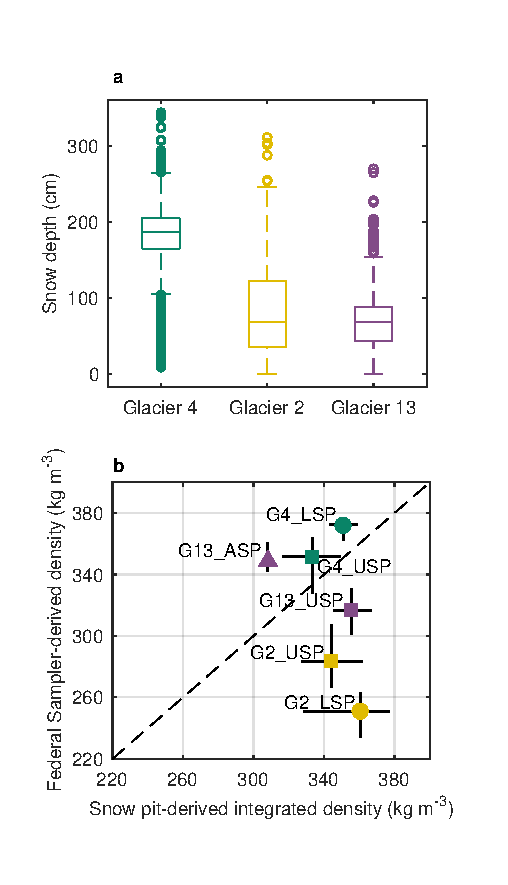
\includegraphics[width =0.35\textwidth]{DepthBoxplot_SPvsFS.pdf}\\
	\caption{Measured snow depth and density. (a) Boxplot of measured snow depth on Glaciers 4, 2 and 13 with the first quartiles (box), median (line within box), minimum and maximum values excluding outliers (bar) and outliers (circles), which are defined as being outside of the range of 1.5 times the quartiles (approximately $\pm2.7\sigma$). (b) Comparison of depth-averaged densities estimated using Federal Sampler measurements (FS) and using a wedge cutter in a snow pit (SP) estimated for Glacier 4 (G4), Glacier 2 (G2) and Glacier 13 (G13). Labels indicate snow pit locations in the accumulation area (ASP), upper ablation area (USP) and lower ablation area (LSP). Error bars for SP-derived densities are calculated by varying the thickness and density of layers that are too hard to sample and error bars for FS-derived densities are the standard deviation of measurements taken at one location. One-to-one line is dashed.}
	\label{fig:DepthBoxplot_SPvsFS}
\end{figure}

\begin{figure*}
	\centering
	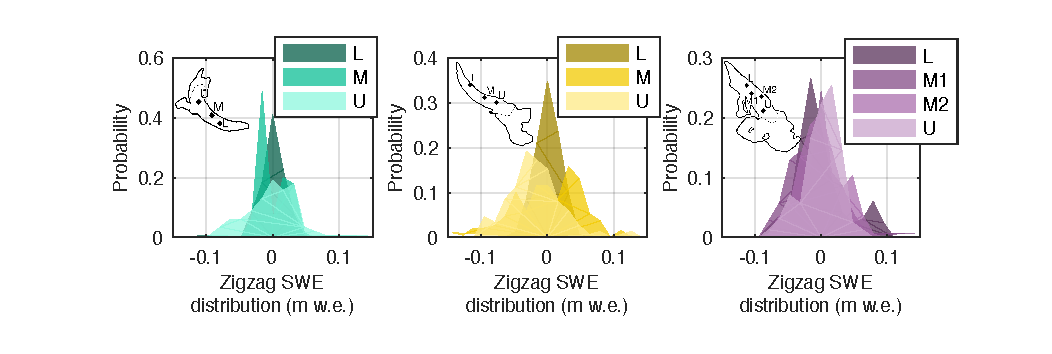
\includegraphics[width =0.95\textwidth]{ZigzagHistogram.pdf}\\
	\caption{Distributions of estimated winter balance values for each zigzag survey in lower (L), middle (M) and upper (U) ablation areas (insets). Local mean has been subtracted. (a) Glacier 4. (b) Glacier 2. (c) Glacier 13.}
	\label{fig:ZigzagHistogram}
\end{figure*}

\subsubsection{Snow depth}
\textcolor{red}{Mean snow depth varied systematically across the study region,} with Glacier 4 having the highest mean snow depth and Glacier 13 having the lowest (Fig. \ref{fig:DepthBoxplot_SPvsFS}). At each measurement location, the median range of measured depths ($3-4$ points) as a percent of the mean local depth is 2\%, 11\% and 12\%, for Glaciers 4, 2 and 13, respectively. While Glacier 4 has the lowest point-scale variability, as assessed above, it also has the highest proportion of outliers, indicating a more variable snow depth across the glacier. \textcolor{red}{The average standard deviation of all zigzag depth measurements is 0.07\,m, 0.17\,m. and 0.14\,m, for Glaciers 4, 2 and 13, respectively. When converted to values of winter using the local FS-derived density measurement, the average standard deviation is 0.027\,m\,w.e., 0.035\,m\,w.e. and 0.040\,m w.e. WB data for each zigzag are not normally distributed about the mean WB value (Fig. \ref{fig:ZigzagHistogram}).}

\subsubsection{Snow density}

Contrary to expectation, co-located FS and SP measurements are found to be uncorrelated (R$^2=0.25$, Fig. \ref{fig:DepthBoxplot_SPvsFS}b). The Federal Sampler appears to oversample in deep snow and undersample in shallow snow. Oversampling by small- diameter (3.2--3.8\,cm) sampling tubes has been observed in previous studies, with a percent error between 6.8\% and 11.8\% \citep[e.g.][]{Work1965, Fames1982, Conger2009}. Studies that use Federal Samplers often apply a 10\% correction to all measurements for this reason \citep[e.g.][]{Molotch2005}. Oversampling has been attributed to slots ``shaving'' snow into the tube as it is rotated \citep[e.g.][]{Dixon2012} and to snow falling into the slots, particularly for snow samples with densities $>$400\,kg\,m$^{-3}$ and snow depths $>$1\,m \citep[e.g.][]{Beaumont1963}. Undersampling is likely to occur due to loss of snow from the bottom of the sampler \citep{Turcan1975}. Loss by this mechanism may have occurred in our study given the isothermal and melt-affected snow conditions observed over the lower reaches of Glaciers 2 and 13. Relatively poor Federal Sampler spring-scale sensitivity also calls into question the reliability of measurements for snow depths $<$20\,cm.

We also found that Federal Sampler density values are positively correlated with snow depth (R$^2= 0.59$). This positive relationship could be a result of physical processes, such as compaction in deep snow and preferential formation of depth hoar in shallow snow, but is more likely a result of measurement artefacts for a number of reasons. First, the range of densities measured by the Federal Sampler is large (227--431\,kg\, m$^{-3}$) and the extreme values seem unlikely given the conditions at the time of sampling. Second, compaction effects of the magnitude required to explain the density differences between snow pit and Federal Sampler measurements would not be expected at the measured snow depths (up to 340\,cm). Third, no linear relationship exists between depth and SP-derived density (R$^2 = 0.05$). These findings indicate that the Federal Sampler measurements have a bias which we have not identified a suitable correction.

\subsection{Density assignment}

Given the lack of correlation between co-located SP- and FS-derived densities (Fig. \ref{fig:DepthBoxplot_SPvsFS}), we use the densities derived from these two methods separately (Table \ref{tab:densityOptions}). SP-derived regional (S1) and glacier-mean (S2) densities are within one standard deviation of the corresponding FS-derived densities (F1 and F2) although SP-derived density values are larger (see Supplementary Material, Table \ref{tab:Density}). For both SP- and FS-derived densities, the mean density for any given glacier (S2 or F2) is within one standard deviation of the mean across all glaciers (S1 or F1). Correlations between elevation and SP- and FS-derived densities are generally high (R$^2>$ 0.5) but vary between glaciers (Supplementary material, Table \ref{tab:Density}). For any given glacier, the standard deviation of the 3--4 SP- or FS-derived densities is $<$13\% of the mean of those values (S2 or F2) (Supplementary material, Table \ref{tab:Density}). We adopt S2 (glacier-wide mean of SP-derived densities) as the reference method of density assignment. Though the method described by S2 does not account for known basin-scale spatial variability in snow density \citep[e.g.][]{Wetlaufer2016}, it is consistent with most winter balance studies, which assume a uniform density for individual glaciers and measure snow density profiles at multiple locations in a study basin \citep[e.g.][]{Elder1991,McGrath2015,Cullen2017}. 

\subsection{Gridcell-averaged winter balance}

The distributions of gridcell-averaged WB values for the individual glaciers are similar to those in Fig. \ref{fig:DepthBoxplot_SPvsFS}a but with fewer outliers. The standard deviation of WB values determined from the zigzag surveys are almost twice as large as the mean standard deviation of point-scale WB values within a gridcell measured along transects. However, a small number of gridcells sampled in transect surveys have standard deviations in WB \textcolor{red}{that exceed 0.25\,m\,w.e. ($\sim$10 times greater than zigzag standard deviations).} We nevertheless assume that the gridcell uncertainty is captured with dense sampling in zigzag gridcells. 

\begin{figure}
	\centering
	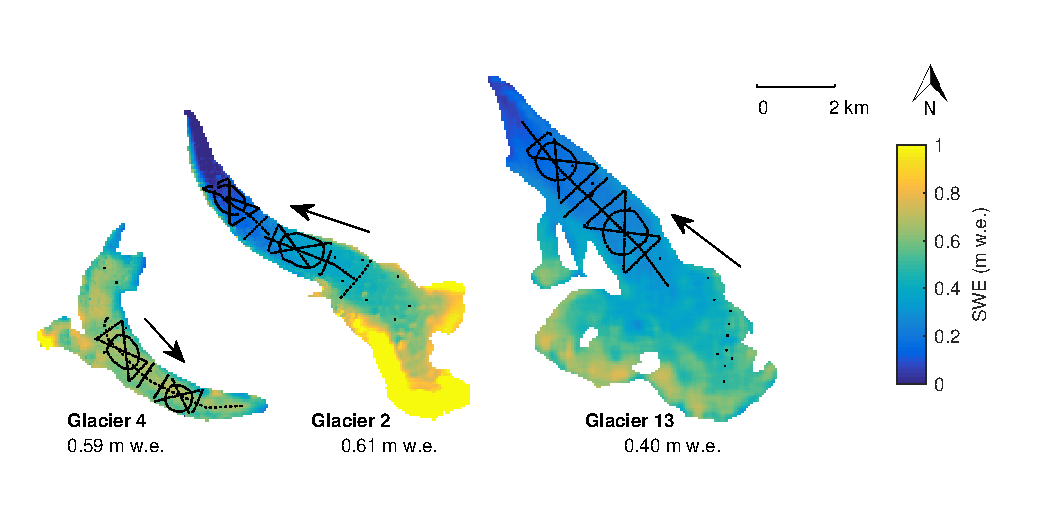
\includegraphics[width =0.5\textwidth]{LR_map.pdf}\\
    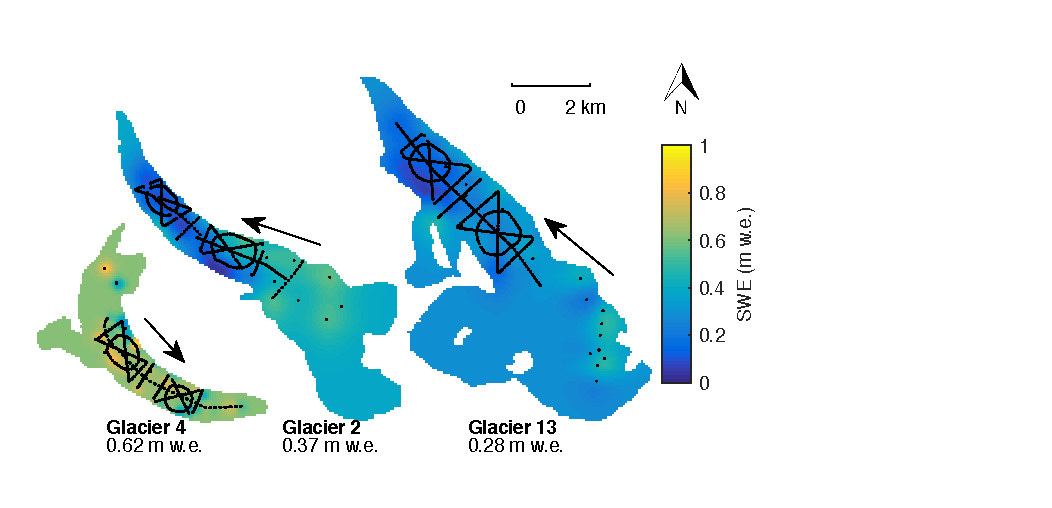
\includegraphics[width =0.5\textwidth]{SK_map.pdf}\\
	\caption{Spatial distribution of winter balance (WB) estimated using linear regression (top row) and simple kriging (bottom row) with densities assigned as per S2 (Table \ref{tab:densityOptions}). Locations of snow depth measurements are shown as black dots. Glacier flow directions are indicated by arrows. Values of glacier-wide WB are given below labels.}
	\label{fig:LR_SK_map}
\end{figure}


\begin{figure}
	\centering
	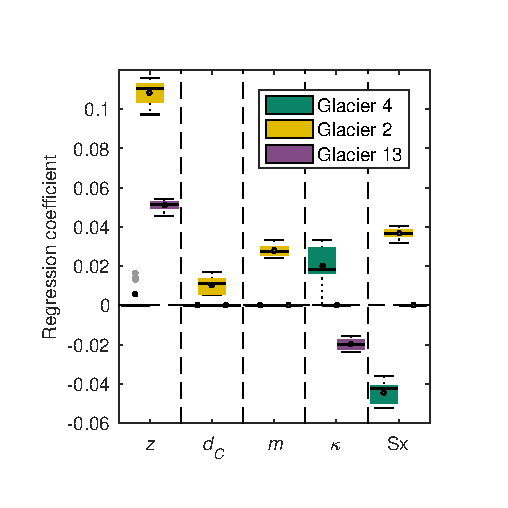
\includegraphics[width =0.4\textwidth]{BetaCoeffs.pdf}\\
	\caption{Distribution of coefficients determined by linear regression of gridcell-averaged WB on gridcell topographic parameters for the eight different density assignment methods (Table \ref{tab:densityOptions}) on each study glaciers. Coefficients are calculated using normalized data resulting in directly comparable coefficient values. Regression coefficients that are not significant are assigned a value of zero. Topographic parameters include elevation ($z$), distance from centreline ($d_C$), slope ($m$) , curvature ($\kappa$) and wind exposure ($Sx$).  Aspect ($\alpha$) and ``northness'' ($N$) are not shown because coefficient values are zero for all interpolation methods. The box shows first quartiles, the line within the box indicates the median, circle within the box indicated mean, bars indicate minimum and maximum values (excluding outliers) and gray dots show outliers, which are defined as being outside of the range of 1.5 times the quartiles (approximately $\pm2.7\sigma$). }
	\label{fig:BetaCoeffs}
\end{figure}


\subsection{Distributed winter balance}
 
 \begin{table}[]
\centering
\caption{Glacier-wide winter balance (WB, m\,w.e.) estimated using linear regression and simple kriging for the three study glaciers. Root mean squared error (RMSE, m\,w.e.) is computed as the average of all RMSE values between gridcell-estimated WB and gridcell-averaged WBs that were randomly selected and excluded from interpolation ($1/3$ of all data). RMSE as a percent of the glacier-wide WB is shown in brackets.}
\label{tab:WSMB&RMSE}
\begin{tabular}{c|cc|cc}
 & \multicolumn{2}{c|}{\textbf{Linear regression}} & \multicolumn{2}{c}{\textbf{Simple kriging}} \\
 & WB & RMSE & WB & RMSE \\ \hline
\textbf{G4} & 0.582 & 0.153 (26\%) & 0.616 & 0.134 (22\%) \\
\textbf{G2} & 0.577 & 0.102 (18\%) & 0.367 & 0.073 (20\%) \\
\textbf{G13} & 0.381 & 0.080 (21\%) & 0.271 & 0.068 (25\%)
\end{tabular}
\end{table}

\begin{figure*}
	\centering
	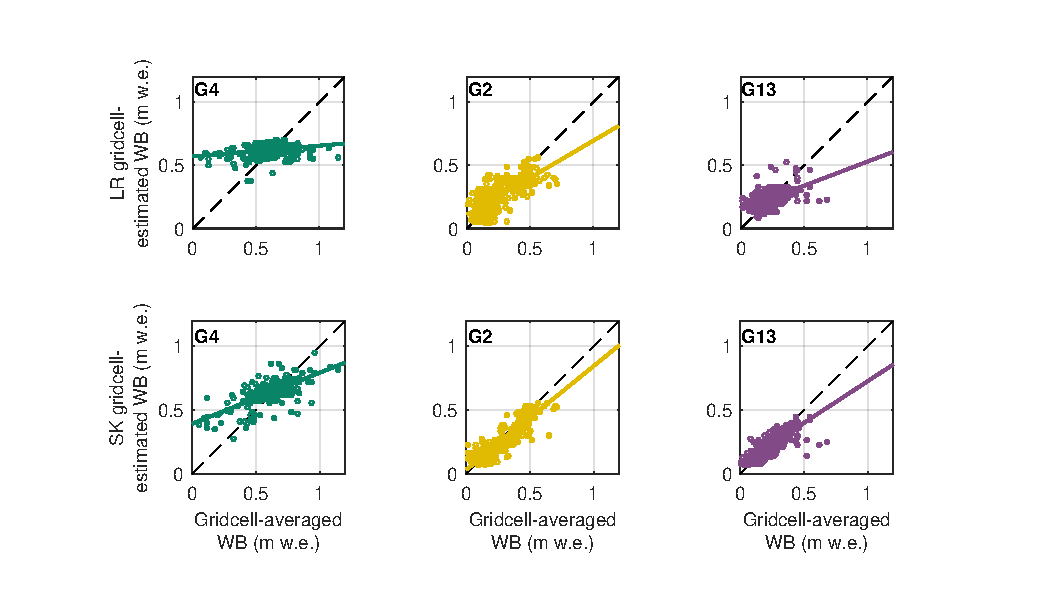
\includegraphics[width =0.7\textwidth]{observedVSestimated_S2.pdf}\\
	\caption{Estimated winter balance (WB) versus WB data. Gridcell-estimated WB is found using linear regression (LR, top row) and simple kriging (SK, bottom row) and is plotted against gridcell-averaged WB along with best fit regression lines for Glacier 4 (left), Glacier 2 (middle) and Glacier 13 (right).}
	\label{fig:observedVSestimated_S2}
\end{figure*}

\begin{figure}
	\centering
	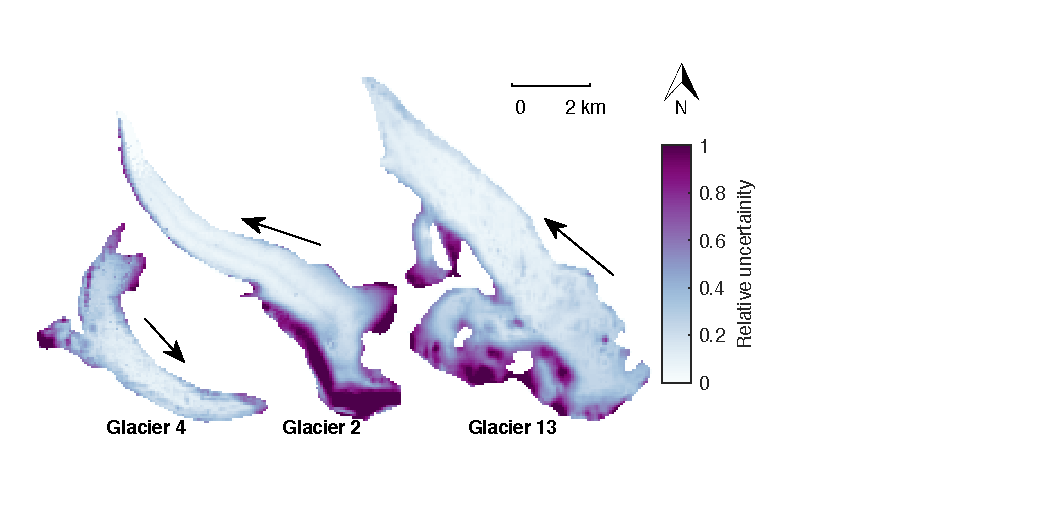
\includegraphics[width =0.5\textwidth]{SpatialVar_LR.pdf}\\
	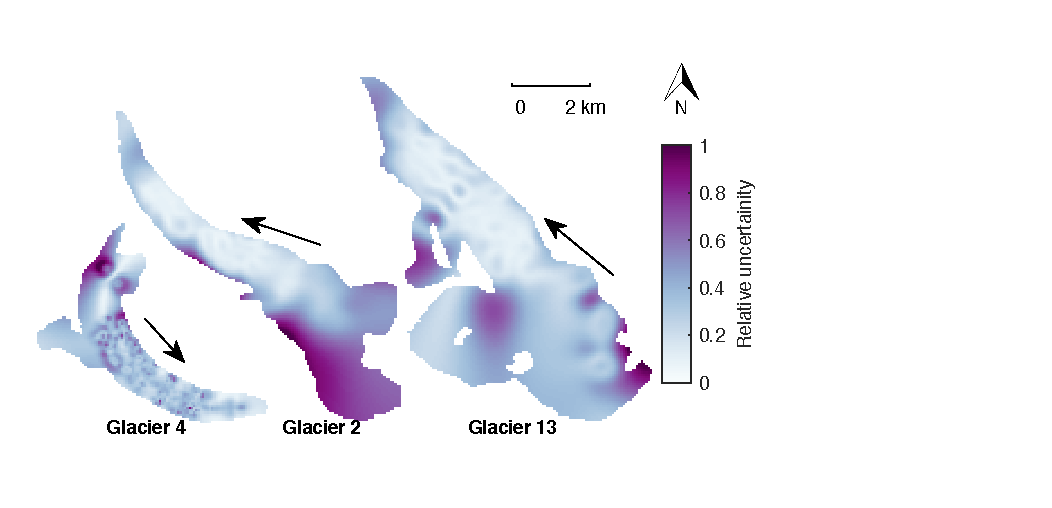
\includegraphics[width =0.5\textwidth]{SpatialVar_SK.pdf}\\
	\caption{Relative uncertainty in gridcell-estimated winter balance (WB) estimated using linear regression (top row) and simple kriging (bottom row). Relative uncertainty is calculated as the sum of differences between every pair of one hundred estimates of gridcell-estimated WB that include grid-scale and interpolation uncertainty. The sum is then normalized for each glacier. Values closer to one indicate higher relative uncertainty. Results for density interpolation method S2 are shown. Glacier flow directions are indicated by arrows.}
	\label{fig:WSMBspatialvar}
\end{figure}

\subsubsection{Linear Regression}

Analysis of topographic parameters reveals that elevation ($z$) is the most significant predictor of gridcell-averaged WB for Glaciers 2 and 13, while wind distribution ($Sx$) is the most significant predictor for Glacier 4 (Fig. \ref{fig:BetaCoeffs}). Gridcell-averaged WB is positively correlated with elevation. It is possible that the elevation correlation was accentuated due to melt onset (1--2 week early), especially on Glacier 13 (Yukon Snow Survey Bulletin and Water Supply Forecast, May 1, 2016). The southwestern Yukon winter snow pack in 2016 was also well below average (Yukon Snow Survey Bulletin and Water Supply Forecast, May 1, 2016), possibly emphasizing effects of early melt onset. Many WB studies have found elevation to be the most significant predictor of WB data \citep[e.g.][]{Machguth2006, McGrath2015}. However, WB--elevation gradients vary considerably between glaciers \citep[e.g.][]{Winther1998} and other factors, such as glacier orientation relative to dominant wind direction and glacier shape, have been noted to affect WB distribution \citep{Machguth2006,Grabiec2011}. There are also a number of studies that find no significant correlation between WB on glaciers and topographic parameters, with highly variable distribution of snow attributed to complex interactions between topography and the atmosphere \citep[e.g.][]{Grabiec2011,Lopez2011}. Linearly extrapolating relationships into unmeasured locations, especially the accumulation area, is most susceptible to large errors (Fig. \ref{fig:WSMBspatialvar}). The accumulation area typically also has the highest WB (Fig. \ref{fig:LR_SK_map}), affecting the glacier-wide WB estimated for the glacier. In our study, the dependence of WB on elevation results in $\sim$1\% of the area of Glacier 2 with gridcell-estimated WB $>$1.5\,m\,w.e. 

Gridcell-averaged WB is negatively correlated with $Sx$ on Glacier 4, counter-intuitively indicating less snow in `sheltered' areas, while gridcell-averaged WB is positively correlated with $Sx$ on Glaciers 2 and 13. Similarly, gridcell-averaged WB is positively correlated with curvature for Glacier 4 and negatively correlated for the other two glaciers. Wind redistribution and preferential deposition of snow is known to have a large influence on accumulation at sub-basin scales \citep[e.g.][]{Dadic2010, Winstral2013,Gerber2017}. Our results indicate that wind likely has an impact on snow distribution but that the wind redistribution parameter may not adequately represent wind effects as applied to our study glaciers. For example, Glacier 4 is located in a curved valley with steep side walls, so specifying a single cardinal direction for wind may not be adequate. Further, the scale of deposition may be smaller than the resolution of the $Sx$ parameter estimated from our DEM. Our results corroborate \cite{McGrath2015}, who undertook a WB study on six glaciers in Alaska (DEM resolutions of 5 m) and found that $Sx$ was the only other significant parameter, besides elevation, for all glaciers. $Sx$ regression coefficients were smaller than elevation regression coefficients and in some cases, negative. Sublimation from blowing snow has also been shown to be an important mechanism mass loss from ridges  \citep[e.g.][]{Musselman2015}. Incorporating snow loss, as well as redistribution and preferential deposition, may be needed for accurate representations of distributed WB. 

While LRs have been used to predict WB in other basins, we find that transfer of LR coefficients between glaciers results in large estimation error. The lowest root mean squared error (0.21\,m\,w.e.) results from estimating a LR using all available observations. Our results are consistent with \cite{Grunewald2013}, who found that local statistical models are able to perform relatively well but they cannot be transferred to different basins and that regional-scale models are not able to explain the majority of observed variance. 

\subsubsection{Simple kriging}

Since simple kriging (SK) is a data-driven interpolation method, the RMSE of gridcell-estimated WB values is lower for SK than LR (Fig. \ref{fig:observedVSestimated_S2} and Table \ref{tab:WSMB&RMSE}). However, the uncertainty in glacier-wide WB that arises from using SK is large, and unrealistic glacier-wide WBs of 0\,m\,w.e. can be estimated. Further, our observations are generally limited to the ablation area, so SK produces almost uniform gridcell-estimated WBs in the accumulation area, which is inconsistent with observations described in the literature \citep[e.g.][]{Machguth2006, Grabiec2011}. Extrapolation using SK leads to large uncertainty (Fig. \ref{fig:WSMBspatialvar}) in estimating WB, further emphasizing the need for spatially distributed point-scale WB measurements in a glacierized basin.

Fitted kriging parameters, including the nugget and spatial correlation length, can provide insight into important scales of WB variability. Glaciers 2 and 13 have longer correlation lengths ($\sim$450\,m) and smaller nuggets, indicating variability at larger scales (see Supplementary Material Table \ref{tab:range&nugget}). Conversely, the model fitted to the SWE data for Glacier 4 has a short correlation length (90 m) and large nugget, indicating that accumulation variability occurs at smaller scales. 

\subsubsection{LR and SK comparison}
 
LR and SK estimate a winter balance of $\sim$0.6\,m\,w.e. for Glacier 4 but both are poor predictors of gridcell-averaged WB at measurement locations (Table \ref{tab:WSMB&RMSE}). For Glaciers 2 and 13, SK estimates are more than 0.1\,m\,w.e. (up to 40\%) lower than LR estimates (Table \ref{tab:WSMB&RMSE}) due to differences in extrapolation. Gridcell-estimated WBs found using LR and SK differ considerably in the upper accumulation areas of Glaciers 2 and 13 (Fig. \ref{fig:LR_SK_map}), where observations are sparse and topographic parameters, like elevation, vary dramatically. The significant influence of elevation in the LR results in substantially higher gridcell-estimated WBs at high elevation, whereas gridcell-estimated WBs found using SK approximate the mean of WB data in these areas. However, when only the ablation area is considered, LR and SK produce gridcell-estimated WBs that differ by less than 7\% for all glaciers. Choice of interpolation method therefore affects how WB data is extrapolated, which has a large effect on glacier-wide WB estimates on our study glaciers. 


\begin{figure*}
	\centering
	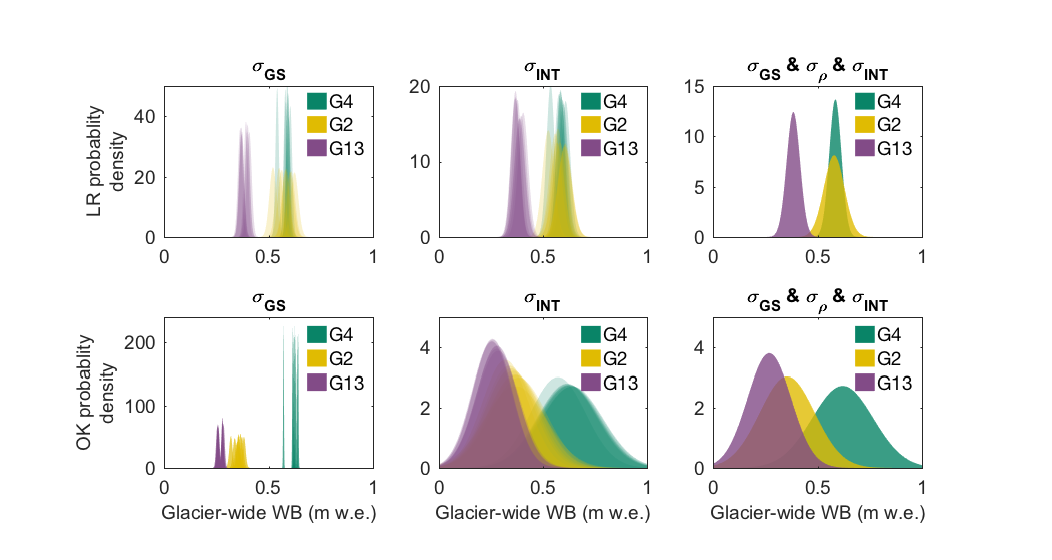
\includegraphics[width =0.95\textwidth]{WSMBDist.pdf}\\
	\caption{Distributions of glacier-wide winter balance (WB) that arise from various sources of uncertainty. (Left column) WB distribution arising from grid-scale uncertainty ($\sigma_{\mathrm{GS}}$). (Middle column) WB distribution arising from interpolation uncertainty ($\sigma_{INT}$). (Right column) WB distribution arising from a combination of $\sigma_{\mathrm{GS}}$, $\sigma_{\mathrm{INT}}$ and density assignment uncertainty ($\sigma_{\rho}$). Results are shown for interpolation by (top row) linear regression and (bottom row) simple kriging. Distributions for each density assignment method are plotted within each panel for Glacier 4 (G4), Glacier 2 (G2) and Glacier 13 (G13).}
	\label{fig:WSMBDist_LR}
\end{figure*}

\subsection{Uncertainty analysis}

Glacier-wide WB is affected by uncertainty introduced when averaging point-scale WBs ($\sigma_{\mathrm{GS}}$), when chosing a density assignment method ($\sigma_{\rho}$), and when interpolating WB data ($\sigma_{\mathrm{INT}}$). We find that when using LR and SK, $\sigma_{\mathrm{INT}}$ has a larger effect on WB uncertainty than $\sigma_{\mathrm{GS}}$ or $\sigma_{\rho}$. In other words, the distribution of glacier-wide WBs that arises from $\sigma_{\mathrm{GS}}$ is much narrower than the distribution that arises from $\sigma_{\mathrm{INT}}$ (Fig. \ref{fig:WSMBDist_LR} and Table \ref{tab:WSMBdistribution_sigma}). The WB distributions obtained using LR and SK overlap for each glacier, but the distribution modes differ (Fig. \ref{fig:WSMBDist_LR}). SK generally estimates lower WB in the accumulation area, which lowers the glacier-wide WB estimate.  Our results caution against using extrapolated data to compare with WB estimates from remote sensing or modelling studies because this may produce misleading results. If possible, comparison studies should use point-scale WB data rather than interpolated WB values. For both LR and SK, the greatest uncertainty in gridcell-estimated WB occurs in the accumulation area (Fig. \ref{fig:WSMBspatialvar}).


 \begin{table*}[b]
\centering
\caption{Standard deviation ($\times10^{-2}$\,m\,w.e.) of glacier-wide winter balance distributions arising from uncertainties in gridcell-averaged WB ($\sigma_{\mathrm{GS}}$), density assignment ($\sigma_{\rho}$), interpolation ($\sigma_{\mathrm{INT}}$) and all three sources combined ($\sigma_{\mathrm{ALL}}$) for linear regression (left columns) and simple kriging (right columns)}
\label{tab:WSMBdistribution_sigma}
\begin{tabular}{c|cccc|cccc}
 & \multicolumn{4}{c|}{\textbf{Linear regression}} & \multicolumn{4}{c}{\textbf{Simple kriging}} \\
\textbf{} & $\sigma_{\mathrm{GS}}$ & $\sigma_{\rho}$ & $\sigma_{INT}$ & $\sigma_{ALL}$ & $\sigma_{\mathrm{GS}}$ & $\sigma_{\rho}$ & $\sigma_{INT}$ & $\sigma_{ALL}$ \\ \hline
\textbf{Glacier 4} & 0.86 & 1.90 & 2.13 & 2.90 & 0.85 & 2.15 & 14.05 & 14.72 \\
\textbf{Glacier 2} & 1.80 & 3.37 & 3.09 & 4.90 & 2.53 & 2.03 & 13.78 & 13.44 \\
\textbf{Glacier 13} & 1.12 & 1.68 & 2.80 & 3.20 & 1.15 & 1.27 & 9.65 & 10.43
\end{tabular}
\end{table*}

Grid-scale uncertainty ($\sigma_{\mathrm{GS}}$) is the smallest contributor to WB uncertainty. This result is likely due to the fact that many parts of a glacier are characterized by a relatively smooth surface, with roughness lengths on the order of centimetres \citep[e.g.][]{Hock2005}. Low WB uncertainty arising from $\sigma_{\mathrm{GS}}$ implies that obtaining the most accurate value of gridcell-averaged WB does not need to be a priority when designing a snow survey. However, we assume that the gridcells selected for zigzag surveys are representative of $\sigma_{\mathrm{GS}}$ across each glacier, which is likely not true for areas with debris cover, crevasses and steep slopes.

Our Monte Carlo analysis did not include uncertainty arising from a number of data sources, which we assume to be encompassed by investigated sources of uncertainty or to contribute negligibly to WB uncertainty. These neglected sources of uncertainty include error associated with SP and FS density measurement, DEM vertical and horizontal error and error associated with estimating measurement locations.


\subsection{Context and caveats}
\subsubsection{Regional winter balance gradient}

The glacier-wide WBs of our three study glaciers (S2 density assignment method), with an uncertainty equal to one standard deviation of the distribution found with Monte Carlo analysis, are: 0.593\,$\pm$\,0.029\,m\,w.e. on Glacier 4, 0.608\,$\pm$\,0.049\,m\,w.e. on Glacier 2 and 0.404\,$\pm$\,0.029\,m\,w.e. on Glacier 13. Although we find considerable inter- and intra-basin variability in WB estimates, our data are consistent with a regional-scale WB gradient for the continental side of the St. Elias Mountains (Fig. \ref{fig:AccumGrad}). WB data are compiled from \cite{Taylor1969}, the three glaciers presented in this paper, as well as two snow pits we dug near the head of the Kaskawulsh Glacier in May 2016. The data show a linear decrease ($-0.024$\,m\,w.e. km$^{-1}$, R$^2=$0.85) in WB with distance from the regional topographic divide between Kaskawulsh and Hubbard Glaciers in the St. Elias Mountains, as identified by \cite{Taylor1969}. While the three study glaciers fit the regional relationship, the same relationship would not apply if just the Donjek Range is considered. We infer that interaction between meso-scale weather patterns and large-scale mountain topography is a major driver of regional-scale WB. Further insight into regional-scale WB trends can be gained by investigating moisture source trajectories and the contribution of orographic precipitation to WB across the St. Elias Mountains. 

\begin{figure}
	\centering
	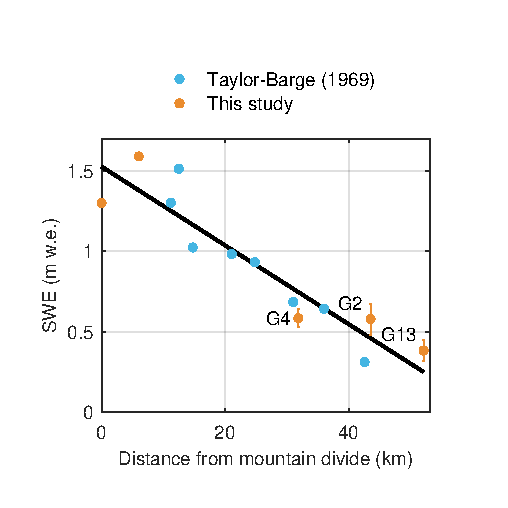
\includegraphics[width =0.35\textwidth]{AccumGrad.pdf}\\
	\caption{Relation between winter balance (WB) and linear distance from the regional topographic divide between Kaskawulsh and Hubbard Glaciers in the St. Elias Mountains. Blue squares are point-scale WBs from snow-pit data reported by \cite{Taylor1969}. Open orange circles, labelled G4, G2 and G13, are glacier-wide WBs estimated with LR and density assignment S2 for Glaciers 4, 2 and 13, with errors bars calculated as the standard deviation of Monte Carlo-derived WB distributions (this study). Filled orange dots are point-scale WBs from snow-pit data at two locations in the accumulation area of the Kaskawulsh Glacier, collected in May 2016 (unpublished data, SFU Glaciology Group). Black line indicates line of best fit (R$^2=0.85$).}
	\label{fig:AccumGrad}
\end{figure}


\subsubsection{Limitations and future work}

Extensions to this work could include investigating experimental design, examining the effects of DEM gridcell size on winter balance and resolving temporal variability. Our sampling design was chosen to extensively sample the ablation area and is likely too finely resolved for many future mass balance surveys to replicate. Determining a sampling design that minimizes error and reduces the number of measurements, known as data efficiency thresholds, would contribute to optimizing snow surveys in mountainous regions. For example, \cite{Lopez2010} concluded that $200-400$ observations are needed to obtain accurate and robust snow distribution models within a non-glacierized alpine basin. 

DEM gridcell size is known to significantly affect computed topographic parameters and the ability for a DEM to resolve important hydrological features (i.e. drainage pathways) in the landscape \citep{Zhang1994, Garbrecht1994, Guo-an2001, Lopez2010}, which can have implications when using topographic parameters in a LR. \cite{Zhang1994} found that a 10 m gridcell size is an optimal compromise between resolution and data volume. Further, the relationship between topographic parameters and WB data is correlated with DEM gridcell size, whereby a decrease in spatial resolution of the DEM results in a decrease in the importance of curvature and an increase in the importance of elevation \citep[e.g.][]{Kienzle2004, Lopez2010}. A detailed and ground controlled DEM is therefore needed to accurately identify features that drive basin-scale WB. Even with a high resolution DEM, small-scale snow variability created by microtopography cannot be resolved. For example, the lower part of Glacier 2 has an undulating ice surface (5 m horizontal displacement and 0.5 m vertical displacement) that results in large variability in snow depth.

Temporal variability in accumulation is not considered in our study. While this limits our conclusions, a number of studies have found temporal stability in spatial patterns of snow accumulation and that terrain-based model could be applied reliable between years \citep[e.g.][]{Grunewald2013}. For example, \cite{Walmsley2015} analyzed more than 40 years of accumulation recorded on two Norwegian glaciers and found that snow accumulation is spatially heterogeneous yet exhibits robust time stability in its distribution. 

%%%%%%%%%%%%%%%%%%%%%%%%%%%%%%%%%%
% CONCLUSION
%%%%%%%%%%%%%%%%%%%%%%%%%%%%%%%%%%
\section{Conclusion}

We estimate winter balance (WB) at various scales for three glaciers (termed as Glacier 2, Glacier 4 and Glacier 13) in the St. Elias Mountains from direct snow depth and density sampling. Our objectives are to (1) critically examine methods of moving from direct snow depth and density measurements to estimating WB and to (2) identify sources of uncertainty, evaluate their magnitude and assess their combined contribution to uncertainty in WB.

We find that interpolating and extrapolating gridcell-averaged WB has a large effect on glacier-wide WB. On Glacier 4, glacier-wide WB is consistent between linear regression (LR) and simple kriging (SK) but both explain only a small portion of the observed variance. This highlights that relatively precise glacier-wide WBs may not necessarily be accurate estimates. On Glaciers 2 and 13, LR and SK are better able to estimate gridcell-averaged WBs but glacier-wide WBs differ considerably between the two interpolation methods due to extrapolation into the accumulation area. Snow distribution patterns are found to differ considerably between glaciers, highlighting strong intra- and inter-basin variability and accumulation drivers acting on multiple scales. Gridcell-averaged WB on Glacier 4 is highly variable, as indicated by shorter range distance, higher nugget value and lower explained variance of gridcell-estimated WB. Glaciers 2 and 13 have lower gridcell-averaged WB variability and elevation is the primary control of observed variation.

For our study glaciers, the glacier-wide WB uncertainty ranges from 0.03\,m w.e (8\%) to 0.15\,m w.e (54\%), depending primarily on the interpolation method. Uncertainty within the interpolation method is the largest source of glacier-wide WB uncertainty when compared to uncertainty in grid-scale WB values and density assignment method. Future studies could reduce WB uncertainty by increasing the spatial distribution of snow depth sampling rather than the number of measurements within a single gridcell along a transect. In our work, increased sampling within the accumulation area would better constrain WB data extrapolation and decrease uncertainty. Despite challenges in accurately estimating WB, our data are consistent with a regional-scale WB gradient for the continental side of the St. Elias Mountains. 

\section{Author contribution statement}

AP organized data collection, performed all calculations and wrote most of the paper. GEF supported data collection, supervised the findings of this work and provided substantial edits to the paper. VR provided guidance with statistical methods and contributed to paper edits.

\section{Acknowledgements}

We thank the Kluane First Nation (KFN), Parks Canada and the Yukon Territorial Government for granting us permission to work in traditional KFN territory and Kluane National Park and Reserve. We are grateful for financial support provided by the Natural Sciences and Engineering Research Council of  Canada, Simon Fraser University, the Northern Scientific  Training  Program and the Polar Continental Shelf Project. We kindly acknowledge Trans North Helicopter pilot Dion Parker, and the Arctic Institute of North America's Kluane Lake Research Station for facilitating field logistics. We are grateful to Alison Criscitiello and Coline Ariagno for all aspects of field assistance and Sarah Furney for data entry assistance. Thank you to Etienne Berthier for providing us with the SPIPT SPOT-5 DEM and for assistance with correcting two DEM sections. We are grateful to Derek Bingham and Michael Grosskopf for assistance with the statistics, including simple kriging. Anonymous reviewers, Luke Wonneck, Leif Anderson and Jeff Crompton all provided
thoughtful and constructive comments on the
manuscript.


%----------------------------------------------------------------------------------------
%	REFERENCE LIST
%----------------------------------------------------------------------------------------
%
\bibliography{/home/glaciology1/Documents/MastersDocuments/MastersLit}
%\bibliography{/Users/Alexandra/Documents/SFU/MastersDocuments/MastersLit}
\bibliographystyle{igs}

%----------------------------------------------------------------------------------------


\end{document}
